% ****** Start of file apssamp.tex ******
%
%   This file is part of the APS files in the REVTeX 4.2 distribution.
%   Version 4.2a of REVTeX, December 2014
%
%   Copyright (c) 2014 The American Physical Society.
%
%   See the REVTeX 4 README file for restrictions and more information.
%
% TeX'ing this file requires that you have AMS-LaTeX 2.0 installed
% as well as the rest of the prerequisites for REVTeX 4.2
%
% See the REVTeX 4 README file
% It also requires running BibTeX. The commands are as follows:
%
%  1)  latex apssamp.tex
%  2)  bibtex apssamp
%  3)  latex apssamp.tex
%  4)  latex apssamp.tex
%
\documentclass[%
 reprint,
%superscriptaddress,
%groupedaddress,
%unsortedaddress,
%runinaddress,
%frontmatterverbose, 
%preprint,
%preprintnumbers,
%nofootinbib,
%nobibnotes,
%bibnotes,
 amsmath,amssymb,
 aps,
%pra,
%prb,
%rmp,
%prstab,
%prstper,
%floatfix,
]{revtex4-2}
\usepackage{lipsum}
\usepackage{graphicx}% Include figure files
\usepackage{dcolumn}% Align table columns on decimal point
\usepackage{bm}% bold math
\usepackage{hyperref}% add hypertext capabilities
\usepackage{xcolor}
\hypersetup{
	colorlinks,
	linkcolor={blue},
	citecolor={red},
	urlcolor={purple}
}
%\usepackage[mathlines]{lineno}% Enable numbering of text and display math
%\linenumbers\relax % Commence numbering lines

%\usepackage[showframe,%Uncomment any one of the following lines to test 
%%scale=0.7, marginratio={1:1, 2:3}, ignoreall,% default settings
%%text={7in,10in},centering,
%%margin=1.5in,
%%total={6.5in,8.75in}, top=1.2in, left=0.9in, includefoot,
%%height=10in,a5paper,hmargin={3cm,0.8in},
%]{geometry}

\begin{document}

\preprint{APS/123-QED}

\title{Study of non-linear optical properties \\using the Z-scan technique}% Force line breaks with \\
%\thanks{A footnote to the article title}%

\author{Maitrey Sharma}
% \altaffiliation[Also at ]{Physics Department, XYZ University.}%Lines break automatically or can be forced with \\
%\author{Second Author}%
% \email{Second.Author@institution.edu}
\affiliation{%
 School of Physical Sciences, National Institute of Science Education and Research, HBNI, Jatni-752050, India.\\
 %This line break forced with \textbackslash\textbackslash
}%

%\collaboration{MUSO Collaboration}%\noaffiliation

%\author{Charlie Author}
% \homepage{http://www.Second.institution.edu/~Charlie.Author}
%\affiliation{
% Second institution and/or address\\
% This line break forced% with \\
%}%
%\affiliation{
% Third institution, the second for Charlie Author
%}%
%\author{Delta Author}
%\affiliation{%
% Authors' institution and/or address\\
% This line break forced with \textbackslash\textbackslash
%}%

%\collaboration{CLEO Collaboration}%\noaffiliation

\date{\today}% It is always \today, today,
             %  but any date may be explicitly specified

\begin{abstract}
\lipsum[1-1]
%\begin{description}
%\item[Usage]
%econdary publications and information retrieval purposes.
%\item[Structure]
%You may use the \texttt{description} environment to structure your abstract;
%use the optional argument of the \verb+\item+ command to give the category of each item. 
%\end{description}
\end{abstract}

%\keywords{Suggested keywords}%Use showkeys class option if keyword
                              %display desired
\maketitle

%\tableofcontents

\section{Introduction}
	In 1875, while working with different solid and liquid dielectrics in an electrostatic field, Scottish physicist John Kerr discovered that those materials were exhibiting double refraction. In other words, the difference in the refractive index, as experienced by the ordinary (perpendicularly polarized) and extraordinary ray (parallel polarized) was proportional to the square of the electric field. This phenomena, of a change in the refractive index of a material in response to an applied electric field, is now known as the \textbf{quadratic electro-optic (QEO) effect} or simply as the \textbf{Kerr effect}.
	\begin{figure}
		\centering
		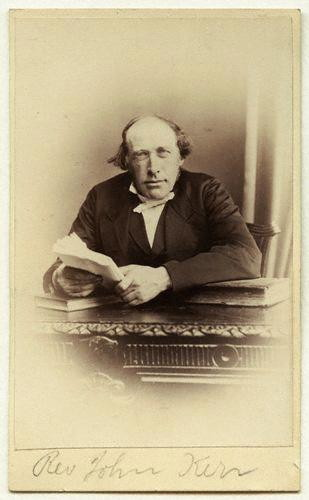
\includegraphics[scale = 0.35]{kerr}
		\caption{John Kerr, c. 1860, photograph by Thomas Annan}
	\end{figure}
	\par
	In the most basic terminology, refractive index of an optical medium defines the ability of that medium to change the path of light. Here, the definition of optical medium is crucial and so is the mathematical description of refractive index. For non-linear optical media, where the polarization density corresponds non-linearly to electric field of the light, the study of the propagation of light becomes quite involved. The principle of superposition, which follows from the Maxwell's equations, is no longer valid as the quantities like electric field are now dependent on parameters like dielectric constant. Non-linear optical media, thus, are remarkable as a plethora of new optical effects can be observed with such materials.
	\par
	On the other hand, a complex refractive index whose real part carries the refractive index and the imaginary part carries the absorption coefficient (also called as \textit{extinction}) can be defined. Now, if a high intensity beam of light is traversed through, the field due to this beam itself can produce changes in the refractive index and absorption coefficients of the material, and if we translate the material as the beam passes through it, we can record the changes as a function of distance. This forms the premise of the experiments that will follow from here, where we will translate materials along the path followed by a Nd-Yag laser beam being focused by a plano-convex lens. The direction in which the sample moves is the $ z $-direction, which gives the name for the technique. As the sample will move across the focus of the laser beam, a characteristic curve will be observed, which can be used to study the non-linear optical properties of the said material.
	



\section{Objectives}
	There are several major objectives that will be achieved as part of this experiment. They are:
	\begin{enumerate}
		\item To study the basics of non-
		linear optical properties by
		using Z-scan technique.
		\item Taking measurements of transmitted power for open and
		closed aperture by translating
		the material in the $ z $-direction.
		\item By fitting these data with the
		appropriate formulas, we will
		find the medium's nonlinear
		absorption coefficient and non-
		linear refractive index for different samples.
		\item To compare the difference between non-linear refractive index of a sample in two forms: as a \textit{thin film coating} and as a \textit{solution}. 
	\end{enumerate}


\section{Theory}
	
	When an electric field is applied across an electric insulator, polarization occurs within the insulator or the dielectric. This polarization density $ P $ is related to the applied electric field $ E $ as
	\begin{equation}
		\mathbf{P} = \varepsilon_0 \chi_e \mathbf{E}
	\end{equation}
	where $ \varepsilon_0 $ is the electric permittivity of free space and $ \chi_e $ is the electric susceptibility of the dielectric. Here, the relation between $ \mathbf{P} $ and $ \mathbf{E} $ is \textit{linear}, and thus the dielectrics which follow this relation are referred to as \textit{linear} (optical) mediums. More generally, for non-linear materials, we can write
	\begin{equation}\label{eq:2}
		\mathbf{P} = \varepsilon_0 \chi^{(1)} : \mathbf{E} + \varepsilon_0 \chi^{(2)} : \mathbf{EE} + \varepsilon_0 \chi^{(3)} : \mathbf{EEE} + \cdots
	\end{equation}
	Here $ \chi^{(n)} $ is the $ n $-th order component of the electric susceptibility of the medium which govern the non-linearities. The `:' symbol represents the scalar product between matrices. When the intensity of the light will be sufficiently high, only then
	these higher order polarization terms will be significant.
	

	\subsection{The Kerr effect}
		For a linear medium, only the first term of equation \eqref{eq:2} is significant and the polarization varies linearly with the electric field. For materials exhibiting a non-negligible Kerr effect, the third, $ \chi^{(3)} $ term is significant, with the even-order terms typically dropping out due to inversion symmetry of the Kerr medium (that is, in media with a center of symmetry).
		\par 
		If the beam of light is reasonably intense, which is true in case of lasers, the beam itself can provide the modulating electric field, without the need for an external field to be applied. Let the electric field $ \mathbf{E} $ in the case be
		\begin{equation}\label{key}
			\mathbf{E} = \mathbf{E}_{\omega} \cos (\omega t)
		\end{equation}
		with $ \mathbf{E_{\omega}} $ being the amplitude of the wave. Combining this with the equation for the polarization, and taking only linear terms and those in $ \chi^{(3)} |\mathbf{E_{\omega}}|^3$, we get
		\begin{equation}\label{key}
			\mathbf{P} = \varepsilon_0 \Big( \chi^{(1)} + \dfrac{3}{4}\chi^{(3)} |\mathbf{E_{\omega}}|^3 \Big) \mathbf{E_{\omega}} \cos (\omega t)
		\end{equation}
		This looks like a linear susceptibility with an additional non-linear term:
		\begin{equation}\label{key}
			\chi = \chi_{\mathrm{LIN}} + \chi_{\mathrm{NL}} = \chi^{(1)} + \dfrac{3}{4}\chi^{(3)} |\mathbf{E_{\omega}}|^3,
		\end{equation}
		and since the refractive index in terms of electric susceptibility is given by $ n = (1 + \chi)^{1/2}$, we have
		\begin{equation}\label{key}
			n = (1 + \chi_{\mathrm{LIN}} + \chi_{\mathrm{NL}})^{1/2} \simeq n_0 \Big( 1 + \dfrac{1}{2n_0^2} \chi_{\mathrm{NL}} \Big)
		\end{equation}
		where $ n_0 = (1 + \chi_{\mathrm{LIN}})^{1/2} $ is the linear refractive index. Using a Taylor expansion since $ \chi_{\mathrm{NL}} \ll n_0^2 $, this gives an \textit{intensity dependent refractive index} (IDRI) of:
		\begin{equation}\label{eq:7}
				n = n_0 + \dfrac{3 \chi^{(3)}}{8 n_0} |\mathbf{E_{\omega}}|^2
		\end{equation}
		As $ I = \frac{1}{2} \varepsilon_0 n_0 c |E_{\omega}|^2$, we obtain
		\begin{equation}\label{eq:8}
			\begin{split}
				n &= n_0 + \dfrac{3}{4} \chi^{(3)} \Big( \dfrac{I}{\varepsilon_0 n_0^2 c} \Big) \\
				\implies n &= n_0 + n_2 I
			\end{split}
		\end{equation}
		where $ n_2  = \frac{3 \chi^{(3)}}{4 \varepsilon_0 n_0^2 c}$  is the nonlinear component of the refractive index. This is known as the \textit{optical Kerr effect}.
	\section{The Self-focusing and self-defocusing phenomena}
		The self focusing (or defocusing) of light beam is due to the
		dependence of the refractive index on the intensity of the beam. From equation \eqref{eq:8}, we
		



		\subsubsection{Wide text (A level-3 head)}
			\lipsum[12-15]


	\subsection{\label{sec:citeref}Citations and References}
		\lipsum[12-15]


		\subsubsection{Citations}
			\lipsum[12-15]




		\subsubsection{Example citations}
			\lipsum[12-15]


		\subsubsection{References}
			\lipsum[12-15]


		\subsubsection{Example references}
			\lipsum[12-15]


	\subsection{Footnotes}%
		\lipsum[12-15]







		\subsubsection{Wide equations}
			\lipsum[12-15]






	\subsection{\label{app:subsec}A subsection in an appendix}
		\lipsum[12-15]

\section{Experimental Set-up}
	\lipsum[16-18]

\section{Experiments}
	\lipsum[19]
	\subsection{Ritwick}
		\lipsum[20]
		\subsubsection{Observations and Results}
			\lipsum[21-25]
	\subsection{SCS}
		\lipsum[20]
		\subsubsection{Observations and Results}
			\lipsum[21-25]
	\subsection{Nanoelectronics Lab}
		\lipsum[20]
		\subsubsection{Observations and Results}
			\lipsum[21-25]
		
\section{Discussions}
	\lipsum[26-30]
\section{Conclusions}
	\lipsum[31-33]


\appendix
\section{Title}
	\lipsum[34-36]
\section{Title 2}
	\lipsum[37-38]
% The \nocite command causes all entries in a bibliography to be printed out
% whether or not they are actually referenced in the text. This is appropriate
% for the sample file to show the different styles of references, but authors
% most likely will not want to use it.
\nocite{*}

\bibliography{apssamp}% Produces the bibliography via BibTeX.

\end{document}
%
% ****** End of file apssamp.tex ******
